\documentclass[a4paper]{report}
\usepackage[utf8]{inputenc}
\usepackage{url}
\usepackage{float}
\usepackage{wrapfig}
\usepackage{graphicx}
\usepackage[toc,page]{appendix}
\graphicspath{ {images/} }
\restylefloat{figure}
\renewcommand*{\thesection}{\arabic{section}}
\renewcommand{\thesubsection}{\thesection(\alph{subsection})}

\begin{document}
\begin{titlepage}
    \begin{center}
        \includegraphics[width=0.7\textwidth]{uol-logo}

        \vspace{5em}

        \Large{COMP390}
        \vspace{1em}
        \Large{\\2020/21}

        \vspace{3em}

        \Large{Generative Adversarial Networks for Terrain Generation}

        \vspace{3em}

        \begin{tabular}{|lp{5.0cm}lll|}
            \hline
                                      &                    &  &   & \\
            \textbf{Student Name:}    & Laura Hulley

            \                         &                    &  &     \\
            \textbf{Student ID:}      & 201277571

            \                         &                    &  &     \\
            \textbf{Supervisor Name:} & Prof Paul Dunne

            \                         &                    &  &     \\
            \hline
        \end{tabular}

        \vspace{3em}

        \LARGE{{\textbf{DEPARTMENT OF\\
                        COMPUTER SCIENCE}}}

        \vspace{2em}

        University of Liverpool\\Liverpool L69 3BX

    \end{center}



\end{titlepage}
\section{Dedication}
\section{AnonTitle}
\section{Abstract}
\section{Contents}
\section{Introduction}
\subsection{Aims and Objectives}
\subsection{Background Information}
\subsubsection{Video Game Terrain}
As the video game industry grows, so does the need for more detailed, exciting and extensive terrains. Procedural terrain generation has been an integral part of video games throughout their existence. An early example of such being the entirely ASCII-based 1980 game, Rogue \cite{rogue}. The level maps, treasure and monsters are procedurally generated each time the game is played. Rogue inspired future games and spawned the category of Rogue-like games which now contains hundreds, if not thousands,\footnote{Figure estimated from Steam search results \cite{roguelikeSteam} and the following list \cite{roguebasin_2020}. There is also the assumption that there are unpublished video games developed using rogue-like techniques.} of procedurally generated games.

The response to the demand for more realistic terrain can be seen in the development of the snowboarding game, SSX(2012) \cite{SSX}. This was the first game in the SSX series to use real world terrain data and the response was overwhelmingly positive. While this was impressive in 2012, it would struggle to compete with the infinite, procedurally generated maps of today's games.

While the terrain in Rogue was formed using simple rule based algorithms, more complex algorithms are needed to create terrain that resembles the natural land forms found on earth. Fractal and noise based techniques can generate incredibly realistic terrain without the limitations of real world data. They offer infinite results and more widely customisable terrain but not without their own drawbacks.

\begin{figure}[H]
    \centering
        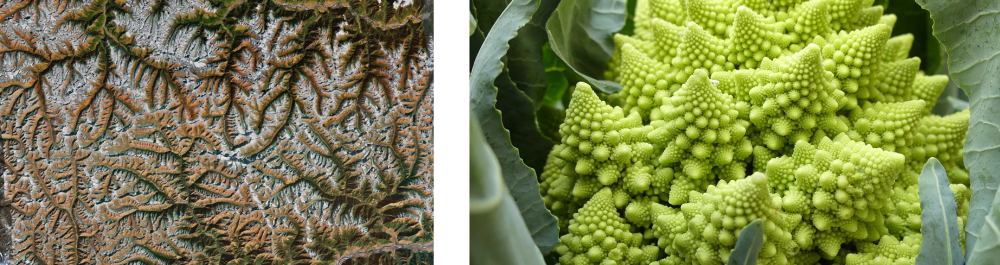
\includegraphics[width=0.95\textwidth]{fractals.png}
        \caption{Shows }
        \label{fig:fractals}
\end{figure}

\paragraph{Fractal Techniques}

Fractals are seen throughout the natural world, from mountains, to rivers, to broccoli (figure \ref{fig:fractals}). Fractals are recursive algorithms that preserve self similarity. In nature, an element of randomness is always present and one algorithm that aims to replicate this is the diamond square algorithm.

The D-Sq algorithm begins with a 2d array, the 4 corners of which are set to some initial values. It then iterates between calculating the midpoint of that square, then the midpoints of the resulting `diamonds'. The values in the array are the `elevation' of the height map and can be plotted in the z axis.

To better understand the algorithm, a simple Python implementation was made which demonstrates the effects of changing the randomness of the algorithm and the resulting `roughness' of the terrain. Figure \ref{fig:fractalPlots} shows the output of the D-Sq script with varying levels of roughness. Two main criticisms of this technique are the presence of artefacts in the resulting terrain and the unrealistic terrain generated (either too regular or too random)\cite{Dsq}. Figure \ref{fig:fractalPlots}(randomness: 5) is an example of the repetitive patterns often generated by this technique. No `mountain' is exactly the same, due to the addition a random value at each iteration, but as a group they can seem unnaturally repetitive. Conversely, with higher levels of roughness or randomness, the mountains can be too steep, sparse and random. Another common problem associated with this technique is the artefacts left behind. Pinches can form between the tiles when the edge values do not line up \cite{proGen}.

\begin{figure}[H]
    \centering
        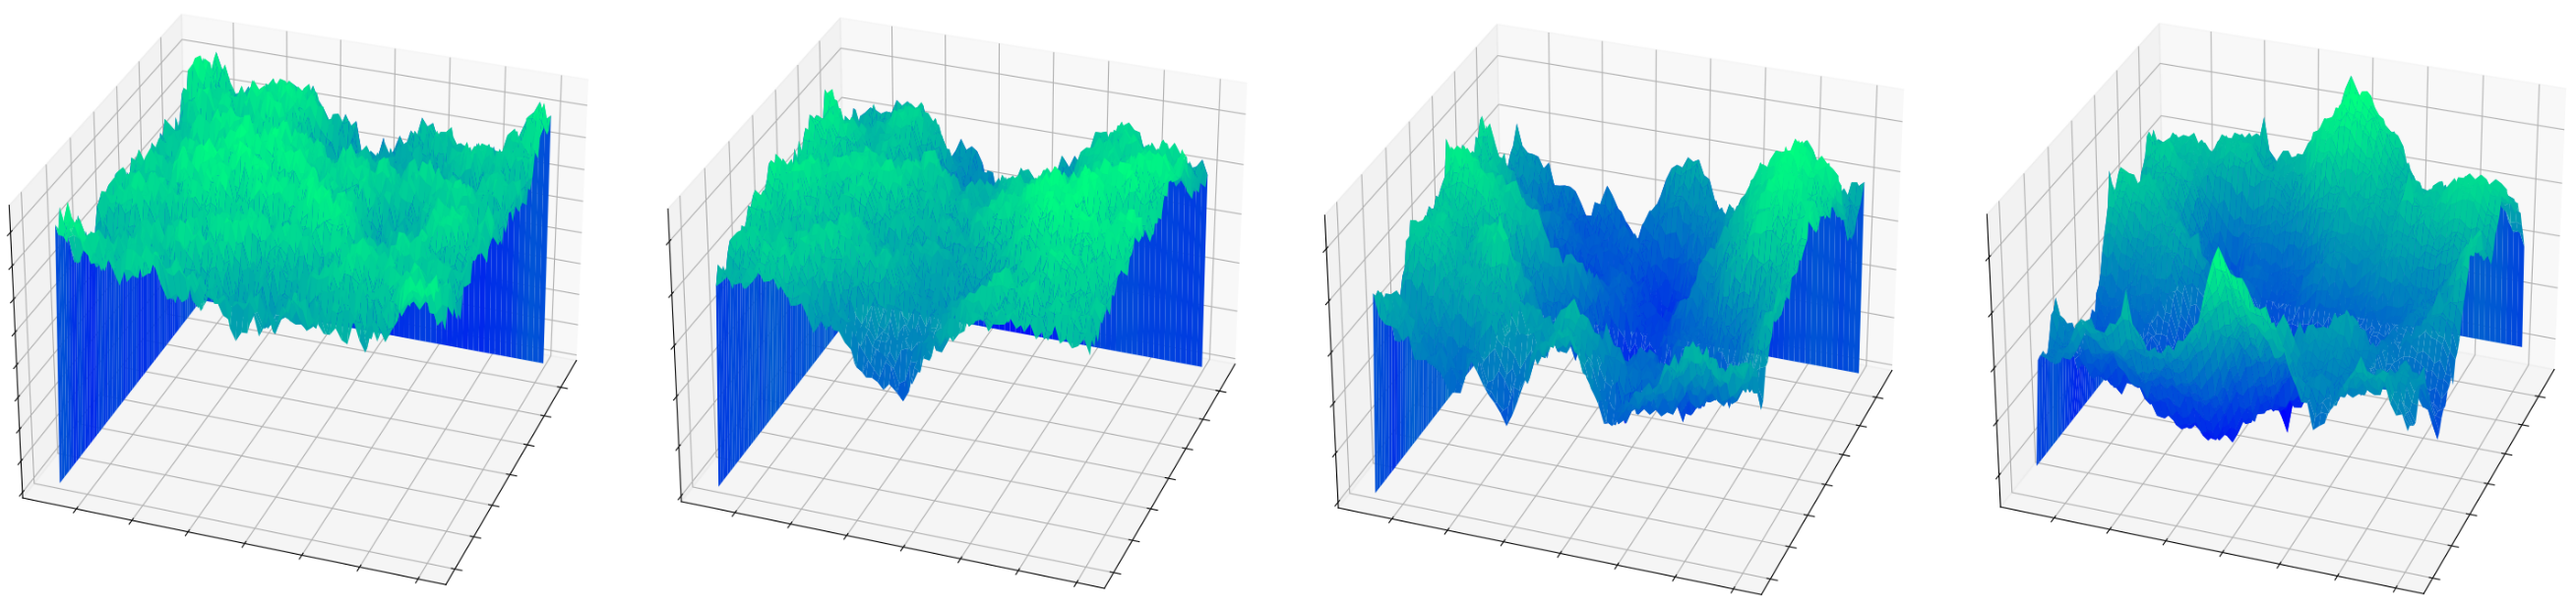
\includegraphics[width=0.95\textwidth]{fractalPlots.png}
        \caption{Shows }
        \label{fig:fractalPlots}
\end{figure}

\paragraph{Noise Techniques}

Another common method of terrain generation involves the use of noise. For Perlin noise, `Noise is determined at point (x,y,z) by computing a pseudo-random gradient at each of the eight nearest vertices on the integer cubic lattice and then doing splined interpolation' \cite{perlinN}. The results can be seen in figure \ref{fig:perlin} (left). Compared to real world height maps (figure \ref{fig:perlin}(right)), the limitations of this technique are clearly visible: the patterns produced are far too regular to appear natural.

The merit of both these techniques is that the style of terrain can easily be changed on a large scale. Small changes to the algorithm, such as changing the range of the random inputs, can produce vastly different terrain (as seen previously: figure \ref{fig:fractalPlots}).

\begin{figure}[H]
    \centering
        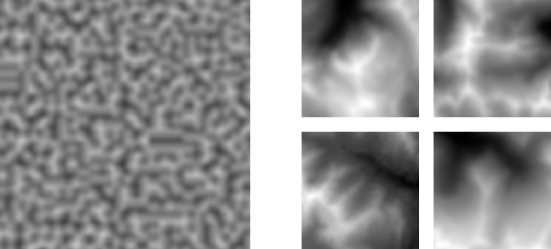
\includegraphics[width=0.95\textwidth]{perlin.png}
        \caption{To Do}
        \label{fig:perlin}
\end{figure}

\paragraph{Combined Techniques}
On their own, fractal and noise techniques will only produce a terrain map with no textures or colouring. To produce a realistic and playable landscape, they must be combined with other algorithms, data or manual input. An example of a software which does just this, is Terragen \cite{terragen}. Decades of development and research into world generation algorithms has resulted in a software that produces incredibly realistic and navigable worlds (figure \ref{fig:terra}). Despite the many complex algorithms and rules used today, the software was originally created using fractal algorithms \cite{Fairc}.

% could talk about ass creed

\begin{figure}[H]
    \centering
        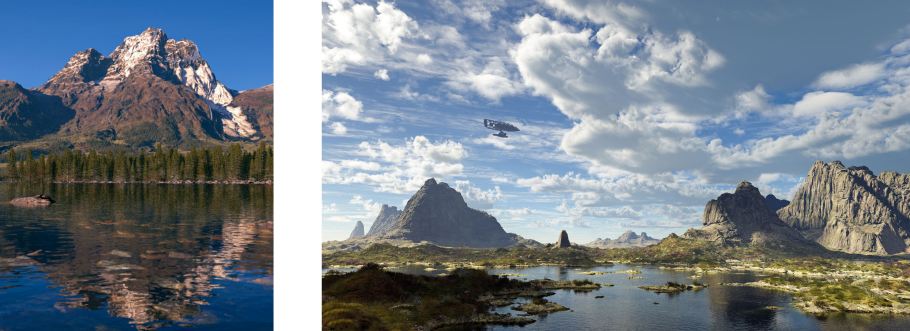
\includegraphics[width=0.95\textwidth]{terra.png}
        \caption{To Do}
        \label{fig:terra}
\end{figure}

\subsubsection{Generative Adversarial Networks}
GANs are a relatively recent development in AI. They were first proposed in a 2014 paper by Ian Goodfellow et. al. \cite{goodfellow2014generative}. Since then, GANs have revolutionised generation and creation in a variety of areas; from creating art in the style of Van Gogh \cite{gangogh} to generating faces of people who do not exist\cite{persondoesnotexist}. While the aforementioned approaches seem lighthearted, they showcase the power of GANs to fool even the human eye.

GANs consist of two competitive networks: A generative network and an adversarial network. The adversarial network is trained (in this case) on real world satellite and elevation data and aims to classify whether an input is an example of real satellite imagery and elevation or a fake (produced by the generator).

The aim of the generator is to `fool' the adversarial network into thinking the data it produces has come from the training set. The input to the generator is a vector from a latent space that it applies a function to, to generate the data that can fool the adversarial network. Both networks are trained simultaneously to avoid either network becoming too good at fooling or classifying the other. The adversarial network is trained on how well it classifies real from fake, whereas the generator is trained on how well its results fool the adversarial. A very basic diagram of a GAN is shown in figure \ref{fig:gan}.

\begin{figure}[H]
    \centering
        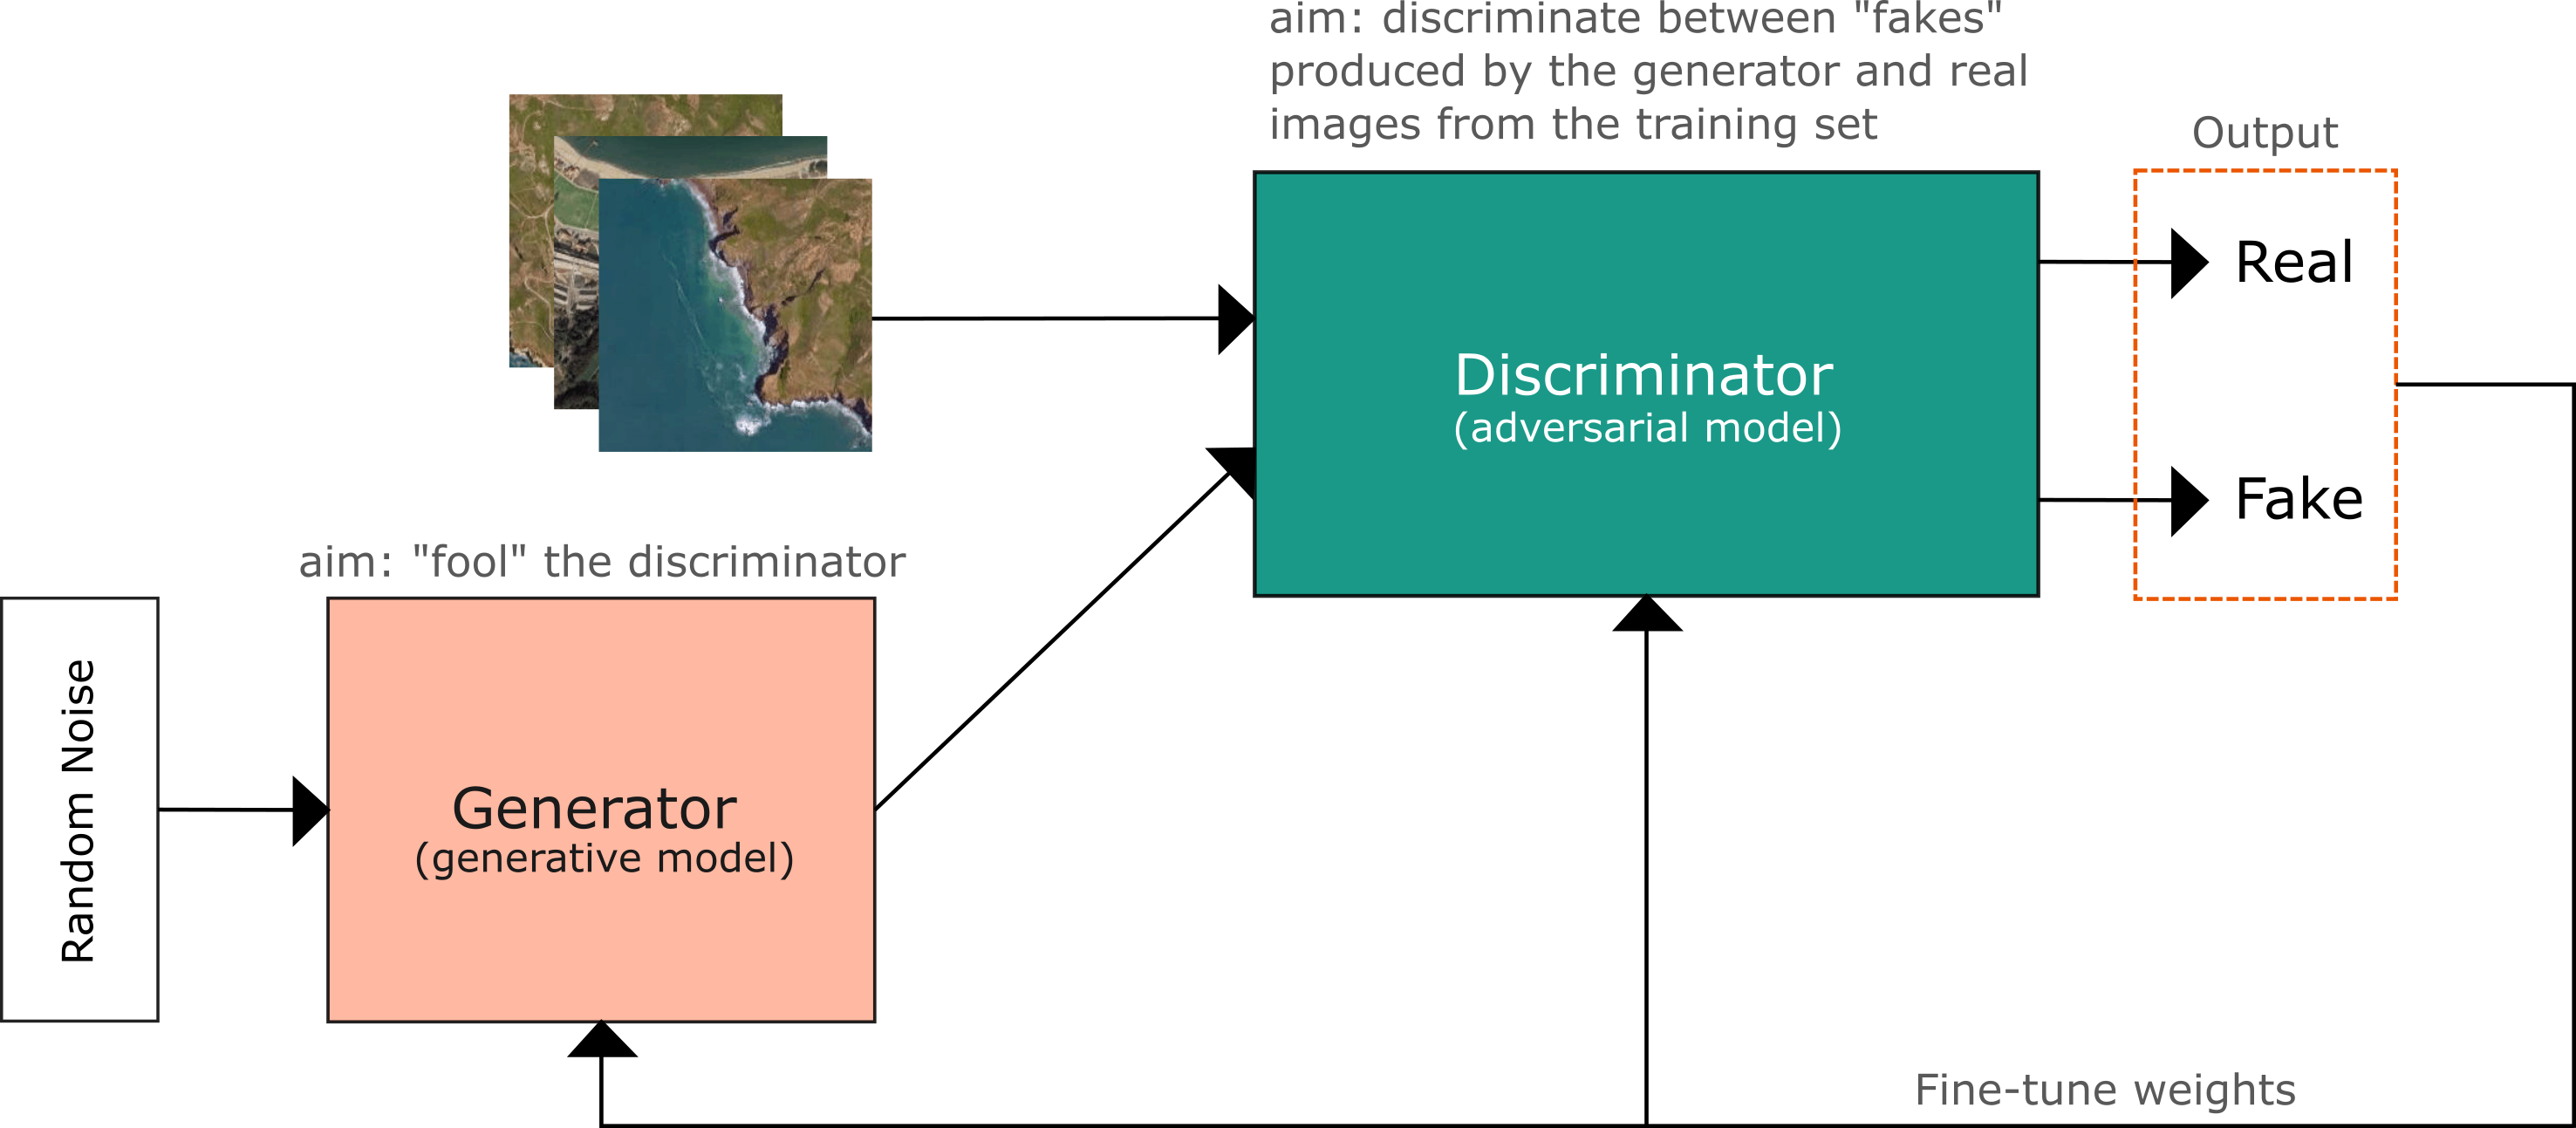
\includegraphics[width=0.95\textwidth]{generator.png}
        \caption{To Do}
        \label{fig:gan}
\end{figure}

\paragraph{StyleGAN}
In March 2019, NVIDIA released StyleGAN: A Style-Based Generator Architecture for Generative Adversarial Networks \cite{ToDo}. This architecture aimed to demistfy aspects of the image synthesis process within the generator network. Before this, studies largely focused on improving the adversarial network; the generative network was more of a `black-box'. The conclusion from this study was that `the traditional GAN generator architecture is in every way inferior to a style-based design'. A variation on StyleGAN2-Ada \cite{ToDo} is the specific GAN architecture used for this project. More information on this architecture and the motivations behind this choice are found in section (ToDo).

\subsection{Existing work}
\paragraph{Terrain Generation with GANs}
Evidence shows the success of GANs in various aspects of terrain generation. Figure \ref{fig:rivers} (left) shows the results of a PGGAN (progressive GAN) trained on satellite images of US rivers \cite{riverSat}. The success of this study opens up the argument for the use of GANs for satellite image generation.

\begin{figure}[H]
    \centering
        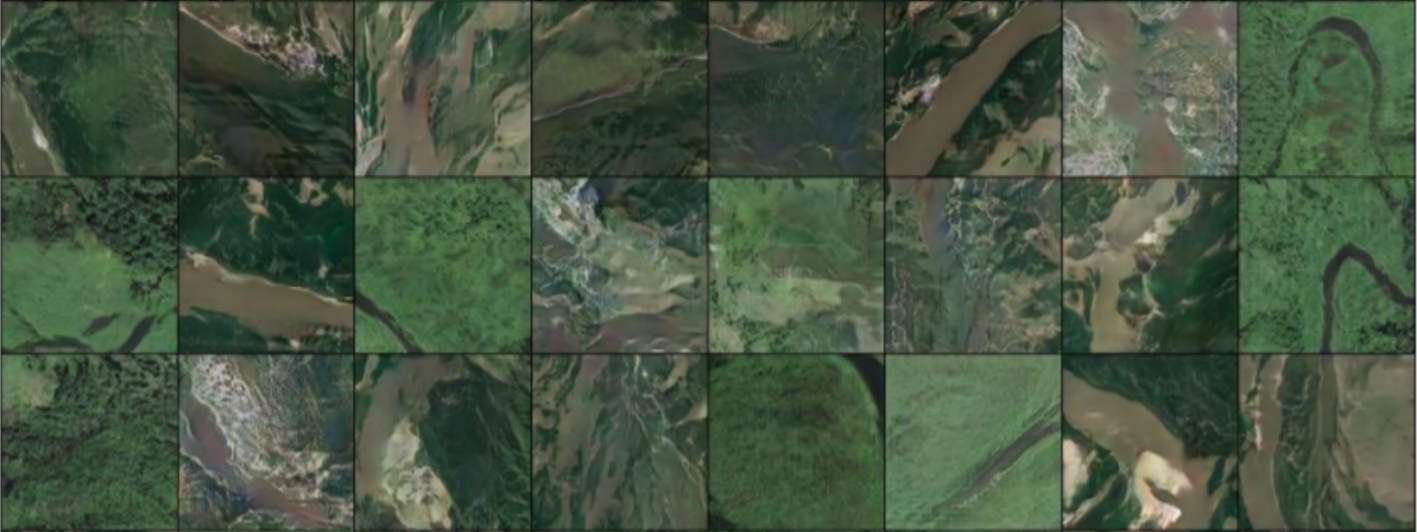
\includegraphics[width=0.9\textwidth]{rivers.png}
        \caption{Shows the results of satellite river generation in \cite{riverSat}}
        \label{fig:rivers}
\end{figure}

As for elevation, a study by Beckham et.al.\cite{beckham2017step} shows similar success generating terrain height maps using NASA elevation data, as seen in Figure \ref{fig:elevs} (left). To texture these height maps, a second generator was used that predicts the colouring for different elevations to varying success (figure \ref{fig:elevs} (right)).

\begin{figure}[H]
    \centering
        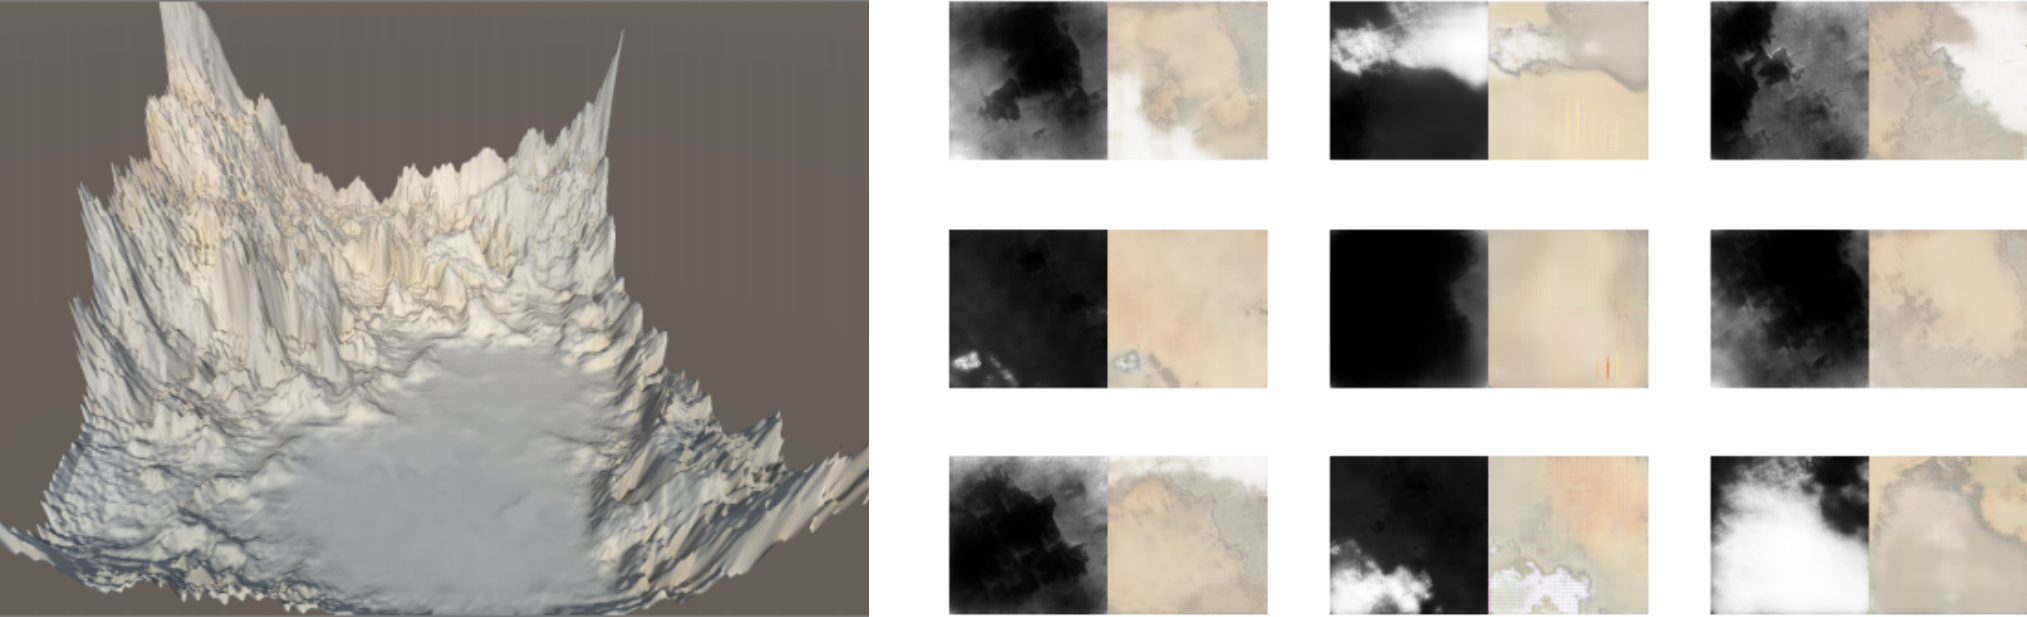
\includegraphics[width=0.9\textwidth]{elevs.png}
        \caption{Shows the results of satellite river generation in \cite{riverSat}}
        \label{fig:elevs}
\end{figure}

Most closely related to my project, is the 2019 paper: `Realistic and Textured Terrain Generation using GANs'. Spick and Walker use a combination of satellite imagery and elevation data to form 4 channel RGBA images that are then used to train a Spatial GAN (SGAN) \cite{ToDo}. The results can be seen in figure \ref{fig:elevGAN}, with further reults listed in the appendix at section \ref{appendix:gan}, figure \ref{fig:elevRes}. These show the ability of SGAN to produce relatively accurate results, especially compared to other models such as DCGAN (a deep convolutional GAN). They also show how even SGAN struggles to capture less common features such as sharp ridges and deep valleys. The SGAN results still show a more smoothed out version of the original terrain data. This is one of the failings that this project aims to address with the use of StyleGAN. 

\begin{figure}[H]
    \centering
        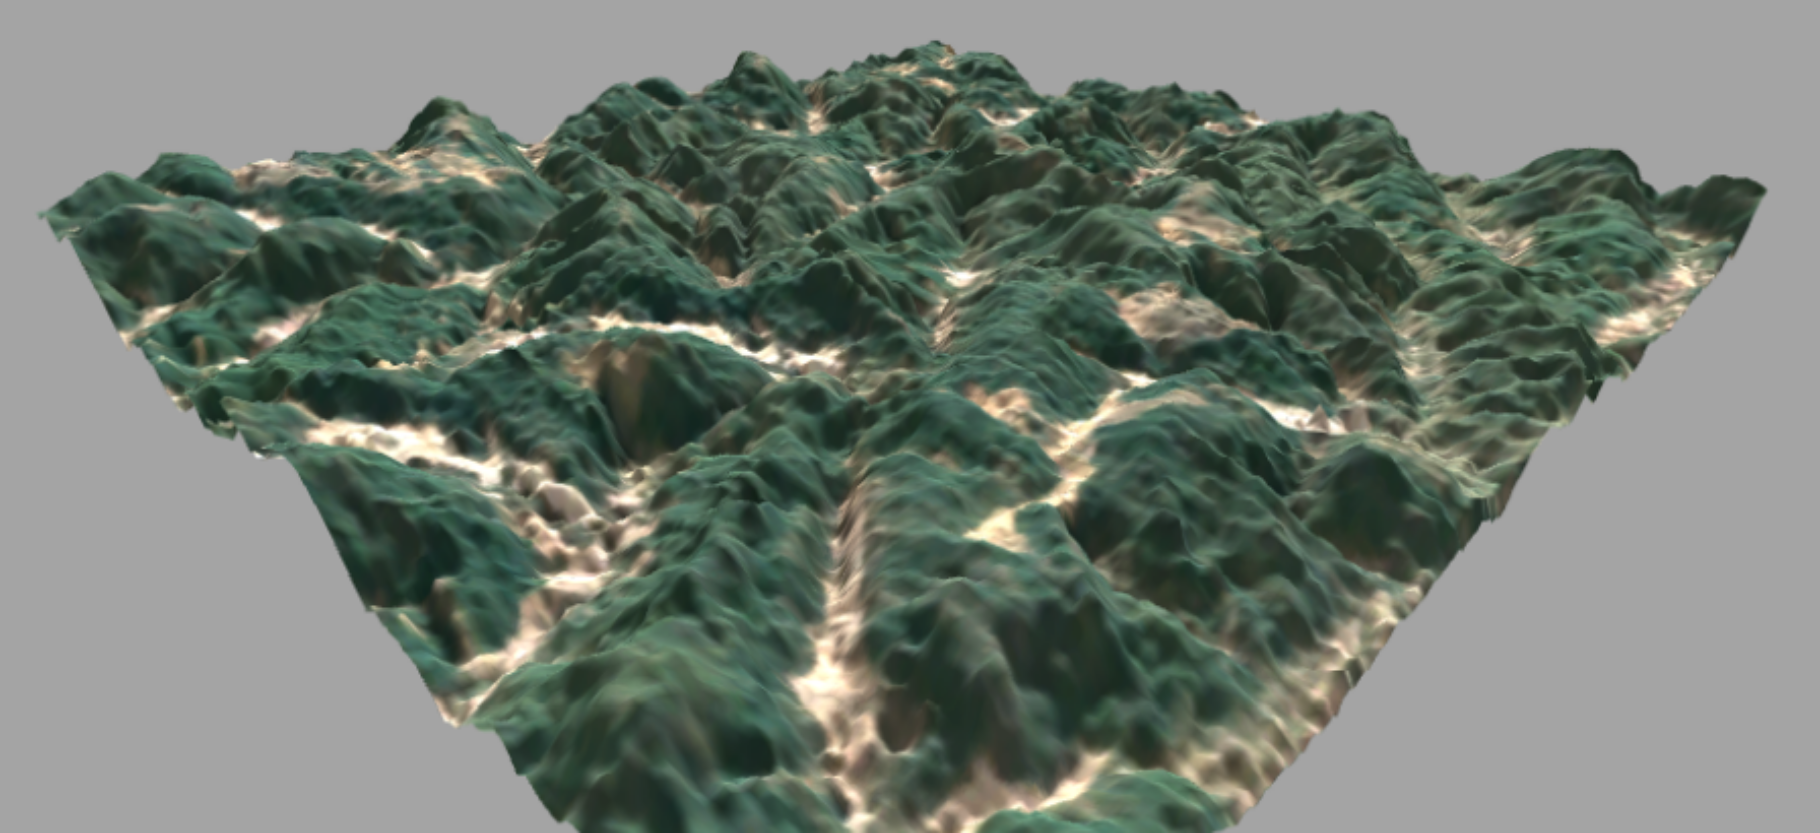
\includegraphics[width=0.9\textwidth]{GANelev.png}
        \caption{Shows the results of satellite river generation in \cite{riverSat}}
        \label{fig:elevGAN}
\end{figure}

\subsection{Motivation}
As mentioned previously, the choice of StyleGAN as the architecture for this model was partly due to the `averaging' of the terrain caused by architectures used in previous studies. StyleGAN is an ideal solution for this as the synthesis of the image can be controlled much more precisely. For the Flickr Faces-HQ data set (figure \ref{fig:ToDo}) this is shown through the ability to control freckles, glasses, hair colour and other stochastic features. In the case of the terrain data in this project, this can be used to control the presence of features such as snow, mountain peaks, or lakes. In the research for this project there was no work found that utilised StyleGAN for combined satellite imagery and elevation data generation.

The traditional methods of fractal and noise based terrain generation have been used and developed upon for decades. The possibility of using GANs as an alternative or supplement to these methods is the main motivation behind this project. StyleGAN addresses many of the points that fractal and noise techniques struggle with, namely the lack of realism and occurrence of artefacts in the resulting terrains.
\section{Design and Implementation}
\subsection{Dataset Creation}
\subsubsection{Requirements}
\begin{enumerate}
    \item The data set should contain enough data to accurately train a model. At least $\sim$2,500 items.
%Ini-tially aimed for  2,500 items however tests showed that reasonable outputscould be produced with as little as 100.
    \item The script for collecting the data should be easy to adapt to collect data from different regions and zoom levels.
    \item The satellite images used should be an appropriate resolution to the chosen zoom levels, so all features are visible in the image.
    \item The elevation accuracy should be appropriate to the zoom levels used in the satellite images.
    \item The script should combine the satellite images and elevation data into a format that can be encoded to an RGBA PNG file.
\end{enumerate}
\subsubsection{Implementation}
The full script used to fetch the data and encode it to PNG files is stored in the get\_data.py file. This script uses the Google Static Maps and Elevation APIs to request the necessary data. Bounding corners of the area to be converted are passed to the script as lat/lng coordinates. The script then iterates through the following loop to convert and save the data as RGBA files.

The process of preparing these files for the model is as follows:
\begin{enumerate}
    \item Select the bounding box of the area to be scanned. For the 128RGBA dataset, an area of the alps shown in figure \ref{fig:alps} was used, bounded by the coordinates NW:47.309535, 8.968262; SE: 46.098575, 14.054704.
    \item Assign the bounding coordinates values to the variables in the script (lines 1 - 5 in algorithm 1).
    \item Set the zoom level and height/ width of the image (12 and 128*128 respectively for 128RGBA). These variables are used by the API to determine the zoom level and size of the returned image. More information on the input options is available in the API docs \cite{ToDo}.
    \item The script then requests the image with the Static Maps API and converts it to a tensor (array).
    \item The \textit{elevations} array is then filled with a single request to the Google Elevations API. If the number of pixels in the image is more than the maximum number of requests allowed to the API, the script interpolates the missing values.
    \item The elevations tensor is normalised to a [0,255] range and concatenated with the image tensor.
    \item The resulting tensor is then encoded to an RGBA PNG image and saved.
\end{enumerate}

\begin{figure}[H]
    \centering
        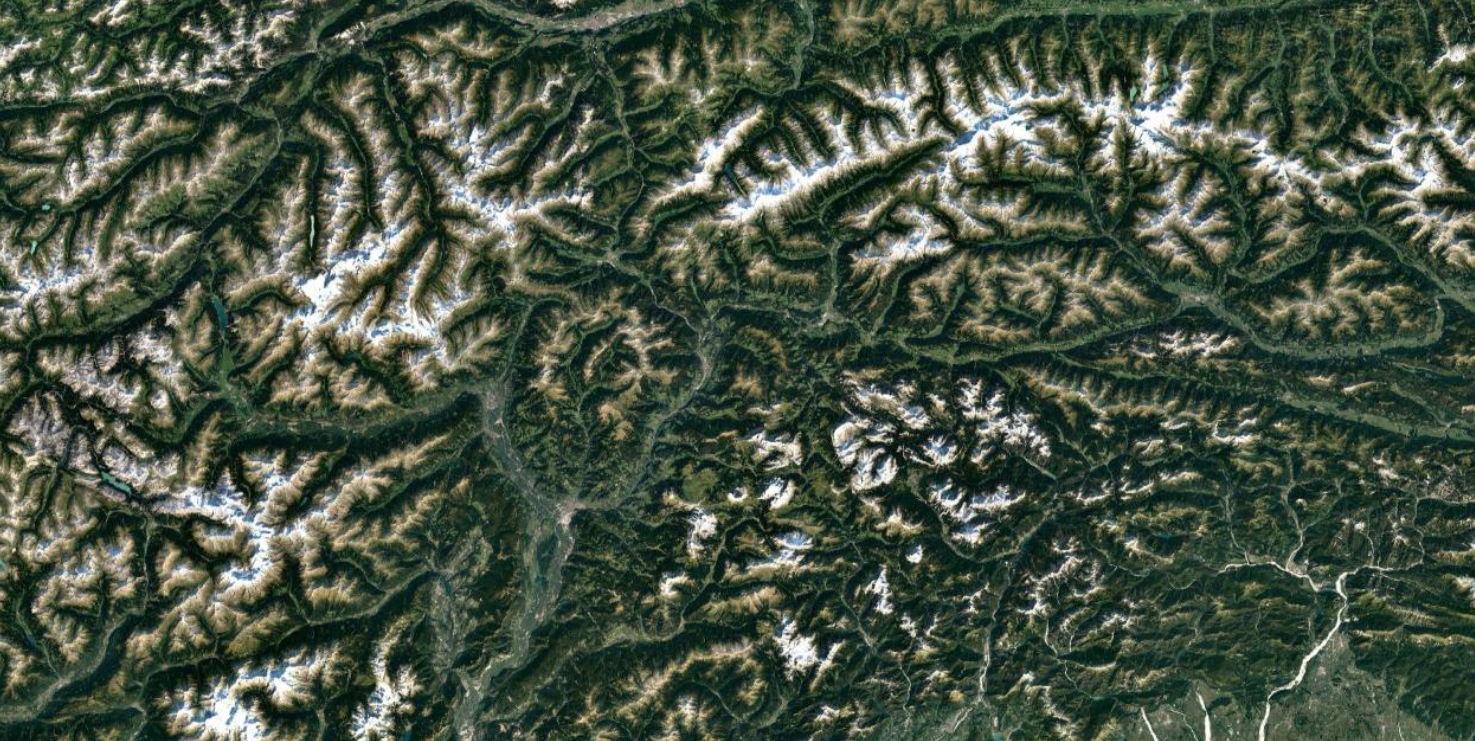
\includegraphics[width=0.95\textwidth]{alps.png}
        \caption{Shows the results of satellite river generation in}
        \label{fig:alps}
\end{figure}

\begin{algorithm}[H]
    \caption{Initialising variables to request and convert data set}
    \begin{algorithmic}[1]
        \State $areaID\gets$ \text{Location as string} \Comment{For file identification}
        \State $northWestLat\gets$ \text{bounding NW latitude}
        \State $northWestLng\gets$ \text{bounding NW longitude}
        \State $southEastLat\gets$ \text{bounding SE latitude}
        \State $southEastLng\gets$ \text{bounding SE longitude}
        \State
        \State $api\_key\gets$ \text{API key} \Comment{\text{from Google Developer Account}}
        \State $zoom\gets$ \text{Chosen zoom level}
        \State $logoHeight\gets$ \text{Height of google logo on image, in pixels}
        \State $picHeight\gets$ \text{y axis length of requested image, in pixels}
        \State $picWidth\gets$ \text{x axis length}
        \State
        \State $numElevations\gets$ \text{num of elevations to be requested (n*n elevations)}
        \State $elevPoints\gets$ \Call{GetElevPoints()}{}
        \State $minE\gets 80000$ \Comment{Max and min elevation in metres}
        \State $maxE\gets -40$
        \State
        \State $mapHeight\gets 256$ \Comment{\text{Lines 18 - 21 are used for Mercator conversion}}
        \State $mapWidth\gets 256$
        \State $xScale\gets 2^{zoom}/(picWidth/mapWidth)$
        \State $yScale\gets 2^{zoom}/(picHeight/mapHeight)$
        \State
        \State $startLat\gets northWestLat$
        \State $startLng\gets northWestLng$
        \State $startCorners\gets$ \Call{GetImageBounds()}{}
        \State
        \State $lngStep\gets startCorners[3] - startCorners[1]$
        \State
        \State $row\gets 0$
        \State $lat\gets startLat$
        \State
        \While{$lat >= southEastLat$}
        \State $lng\gets startLng$
        \State $col\gets 0$
        \While{$lng <= southEastLng$}
        \If{\Call{CheckIfLand}{lat,lng}$\equiv True$}
        \State $bounds\gets$ \Call{GetImageBounds()}{}
        \State $image\gets$ \Call{RequestImage()}{}
        \State $elevSteps\gets$ \Call{GetElevStep()}{}
        \State $elevations\gets$ \Call{RequestElevations()}{}
        \State \Call{CreateTensor()}{}
        \EndIf
        \State $col\gets col+1$
        \State $lng\gets lng + lngStep$
        \EndWhile
        \State $row\gets row-1$
        \State $lat\gets lat + $ \Call{GetLatStep()}{}
        \EndWhile
    \end{algorithmic}
\end{algorithm}

\subsubsection{Development Environment}
The data set creation script was written in Python, in the VS Code editor. Version control is done with Git and the repository for the script (and all of these files) can be found here \cite{ToDo}. Pipenv \cite{ToDo} is used as a packaging tool to ensure this code can be run easily on any machine and mitigate any risk of hardware failure.\footnote{Information on package versions necessary to run the script are available in the pipfile.}

\subsubsection{Design Choices}
\paragraph{File Format - RGBA}
The majority of GAN architectures that were considered for this projected accepted a PNG file as input. A PNG image is typically a 3 channel RBG image: red, green and blue. RGBA is a more uncommon colour format but would work perfectly in this case. The 4th channel, alpha, is used to denote the transparency of the image. For this dataset however, this value is instead used to store the associated elevation data for each pixel. Figure \ref{fig:rgba} shows the structure of each instance in the dataset. The data is formed of 3 dimensional arrays of size (picHeight, picWidth, 4) where pic height and width are the respective size of the image in pixels. Each pixel then has the 4 aforementioned channels associated with it: red, green, blue and alpha (elevation).

There is one main limitation to this format, the values must all be stored as integers. A compromise had to be made to either sacrifice the context of the elevation for the sake of an accurate gradient or vice versa. With a range of -40 to 8,000 metres, it was unlikely the accurate gradients would remain if the values were converted to integers. Because of this, the decision was made to forgo the context of the elevations and instead normalise the elevations from each individual image to a [0,255] range\footnote{This is the range of each of the colour channels of the image. Normalisation to a [-1,1] scale is done as part of the preprocessing of the GAN model.} before casting to integers.

\begin{figure}[H]
    \centering
        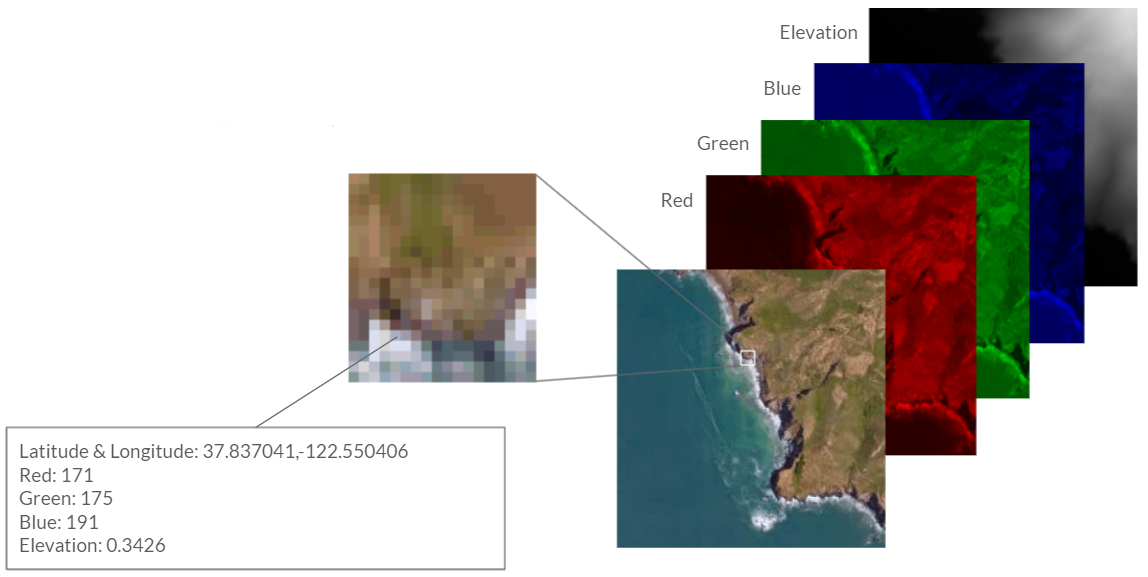
\includegraphics[width=0.95\textwidth]{rgba.png}
        \caption{Shows the results of satellite river generation in}
        \label{fig:rgba}
\end{figure}

\paragraph{Translation From Lat/Lng to Pixel Coordinates}
The Google Static Maps API takes a centre lat/lng as input and outputs a single png image with no accompanying information. One of the biggest obstacles in this project was finding the lat/lng coordinates of the corner of the images in order to request the elevations. There is limited information publicly available about Google's conversion methods but a solution was found using the mercator projection, as seen in the \textit{PointToLatLng()} and \textit{LatLngToPoint()} functions in the get\_data.py file.
The difficulties surrounding this conversion led to the creation of a more general script \cite{ToDo} for tiling Maps API results, to avoid others facing the same struggle.

\paragraph{Region Selection}
The alpine region pictured in figure \ref{fig:alps} was chosen for a number of reasons. It was important to generate a similar terrain to that of the examples shown in figures \ref{fig:fractalPlots}, \ref{fig:rivers}, \ref{fig:elevs} and \ref{fig:elevGAN} in order to form a comparison. The fractal property of the terrain also allows us to compare against the fractal technique, without the need for a texture comparison.

The presence on snow in less than half of the images allows an evaluation of the ability of StyleGAN to generate varied data, and not just learn from the averages. It can also be used to assess how well the model has learned the correlation between snow and higher elevations.

\paragraph{API Limitations and Array Interpolation}
The majority of limits on the APIs were high enough that they did not affect this project. However, the elevation API only allowed 512 locations per request. $\sim$500 elevation points spread across the image was still within the error margin of Google's elevation data. For this reason the decision was made to find the elevation of an even spread of points across the image and interpolate between these points to form the full array necessary for a complete image. Figure \ref{fig:interpolate} shows the different methods of interpolation tested for the elevation array. `Nearest' uses the nearest available value so the resulting heightmap appears more pixelated. The `Linear' and `Cubic' methods both showed similar results however Linear appeared to smooth out some of the natural ridges so Cubic was chosen instead.

\begin{figure}[H]
    \centering
        
\includegraphics[width=0.95\textwidth]{interpolate.png}
        \caption{Shows the results of satellite river generation in}
        \label{fig:interpolate}
\end{figure}

\subsubsection{Evaluation against requirements}
The main dataset used to train the GAN was a set of 2,500 128*128 RGBA PNG images, shown in figure \ref{fig:data}. It took around 2 hours for the script to request, format and save this data. In the run up to this, datasets of different regions, resolutions and zoom levels were created, some of which were tested on the GAN (section ToDo). The format of the script meant it was easy to change the variables used and the elevation and API requests were automatically reformatted accordingly.

\begin{figure}[H]
    \centering
        \includegraphics[width=0.95\textwidth]{data.png}
        \caption{Shows the results of satellite river generation in}
        \label{fig:data}
\end{figure}

\subsection{GAN}
\subsubsection{Requirements}
As listed in the original aims of the project, the aim of the GAN was to generate realistic data that is indistinguishable from the data found in the training set. This data should be suitable to form a comparison between GANs and traditional techniques as methods of terrain generation.

\subsubsection{Implementation}
The specific GAN architecture used was a variation of StyleGAN2-ada \cite{ToDo}, developed by Vadim Epstein. StyleGAN2 was chosen as the architecture for this project as it has significantly better results than the original model for training on datasets with less that $\sim$30k images. It also boasts faster training, less GPU memory consumption alongside the benefits of the original StyleGAN model mentioned previously (section ToDo). The variation developed by Epstein also added support for 4 channel RGBA images so there were minimal changes to the existing code needed.

\subsubsection{Development Environment}
Initially, it was intended for the code to be run on a personal machine. There were obvious hardware limits with this method and the code was run in a Google Colab notebook instead. Google Pro provides access to a P-100 or V-100 Tesla GPU which enabled quick training times and could be left running in the background. The input dataset, generated images, and snapshots of the model throughout training were all automatically stored on Google Drive so there was no risk of data loss.

\subsubsection{Post-processing}
The data generated by the GAN is in the form of RGBA images. This was the best format for the model but they are not ideal for visualising the resulting terrain. A second script, split\_images.py was written that splits the RGBA image into a coloured 3 channel RGB satellite image and a 1 channel greyscale image for the heightmap. These are then converted to raw files and manually loaded into unity to model the terrain.
\subsection{Reflections on the development process}
The vast majority of the development time was spent on the creation of the dataset and this is arguably just as important as the development of the GAN. There was no dataset of this format freely available online so constructing this dataset was almost a project in itself. One of the main results presented in the original StyleGAN paper \cite{ToDo} was a new dataset of high quality portrait photos.

A lot of dead ends had to be hit to achieve the software necessary for this project. For the data set development, these are destailed in the `design choices' section. For the GAN, the largest chunk of the time was spent finding an appropriate architecture and setting up the devleopment environment. Originally a lot of time was spent editing the code of StyleGAN2 to accept 4 channel images, before realising that this variation had already been developed.
\section{Testing}
\begin{figure}[H]
    \centering
        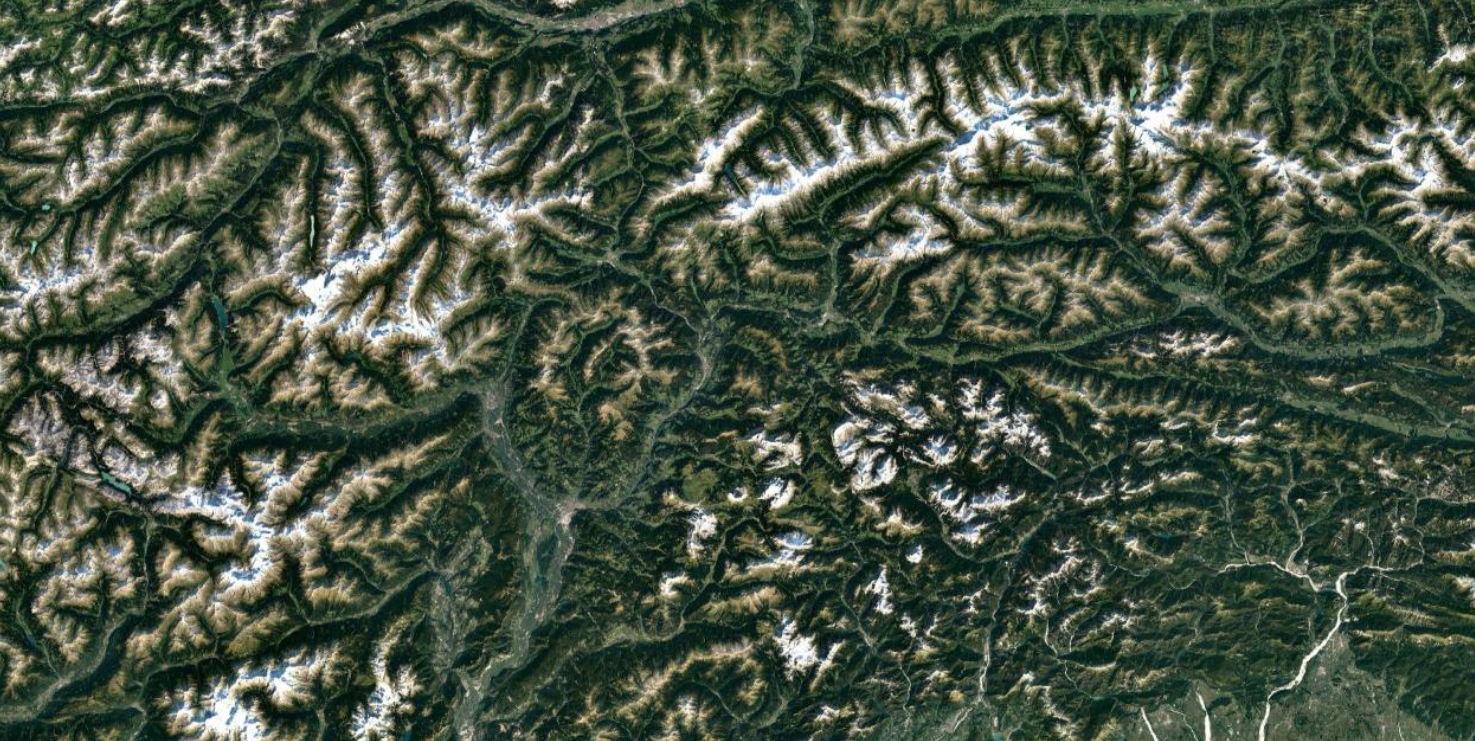
\includegraphics[width=0.95\textwidth]{alps.png}
        \caption{Nice unity model here!}
        \label{fig:ToDo}
\end{figure}

The GAN model was run on different dataset sizes, resolutions and formats. The resulting data was then converted to animated GIFs, 3D unity models or left as static PNG files. The results of these tests for each dataset are listed below.

\subsection{128*128 RGB Dataset}

This is the easiest dataset to see results as the images are clearly visible to the human eye without the transparency channel. The first run to test the model was done with a dataset of only 50 images and still produced impressive results after 280 epochs \footnote{The seemingly random choice of epochs are largely due to being cut off from the Google GPU. When the WiFi cuts out (which it often does), the training has to be restarted from the most recent save point. This takes time and the results are often already visible by the time it cuts out. For smaller test datasets such as this one, it was not necessary to continue training for many more epochs.}(figure \ref{fig:RGB48}).

\begin{figure}[H]
    \centering
        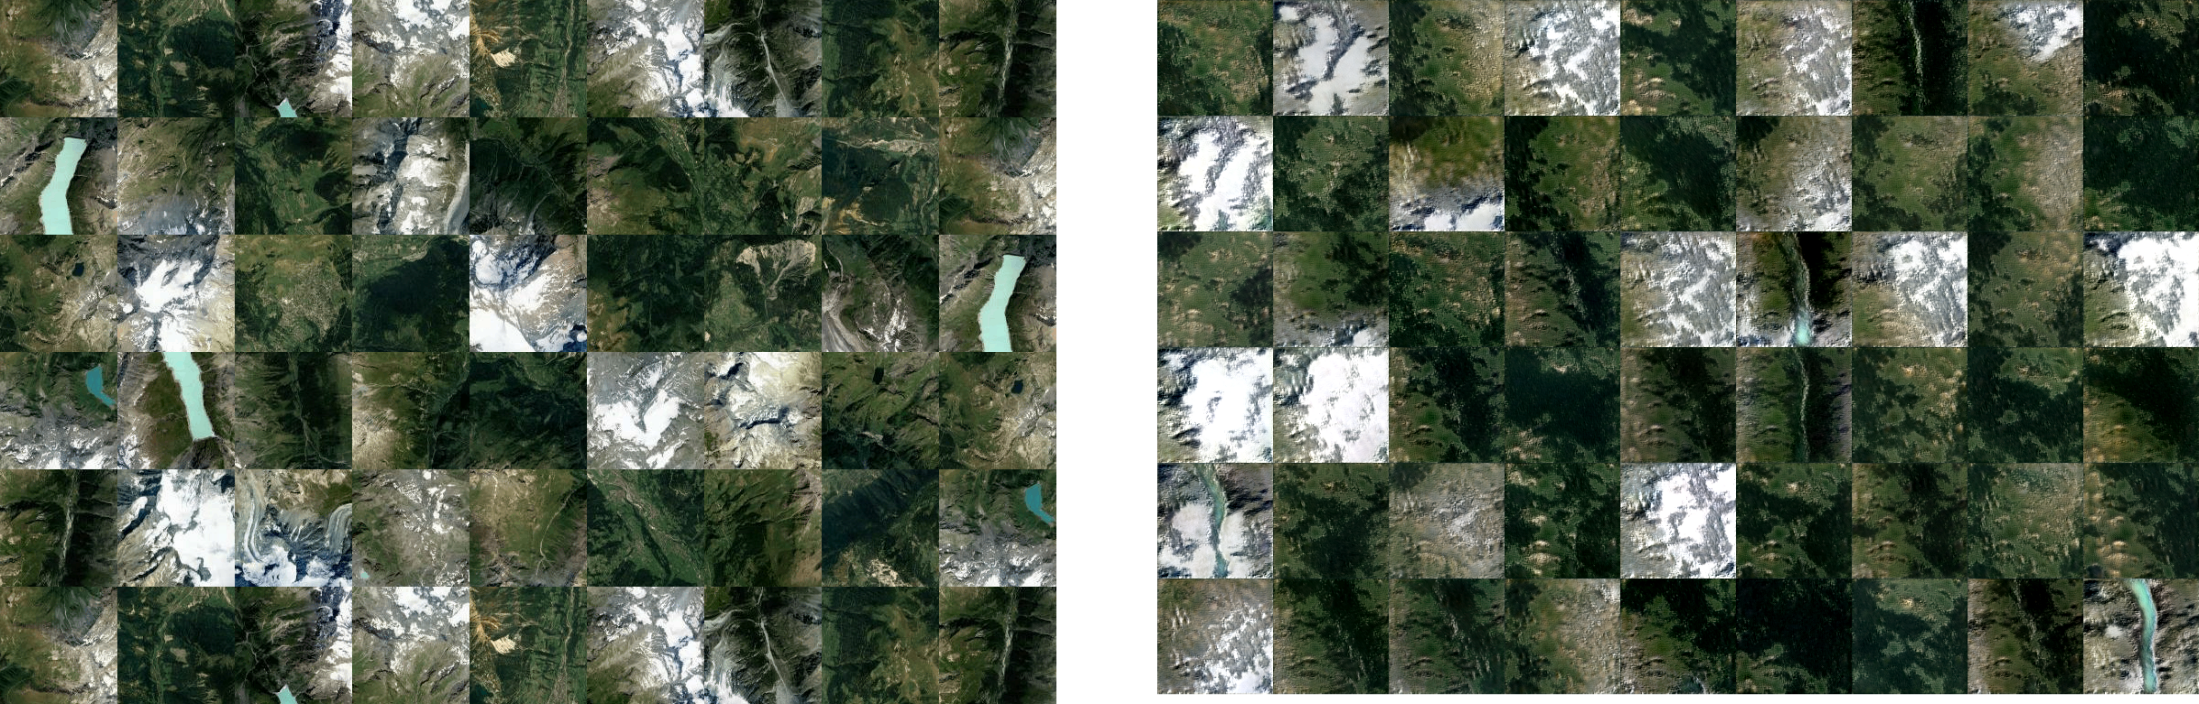
\includegraphics[width=0.95\textwidth]{RGB48.png}
        \caption{Orig 48 dataset and resulting fake}
        \label{fig:RGB48}
\end{figure}

This confirmed the model would be able to train in a reasonable time on a relatively small dataset. The model was then trained on the finished dataset of 2,500\footnote{The data pre-processing script within the StyleGAN2 code automatically mirrors the images. The dataset numbers listed in this section do not account for this, so the model was trained on 5,000 images in this case.} images and trained for 1,200 epochs resulting in figure \ref{fig:ToDo} as output.

\begin{figure}[H]
    \centering
        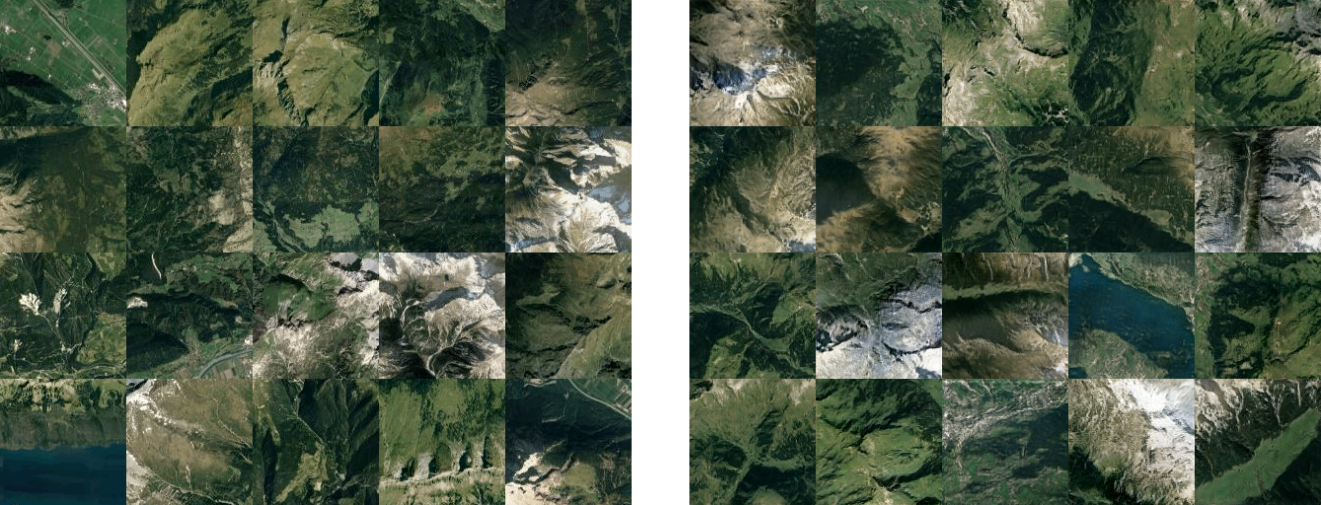
\includegraphics[width=0.95\textwidth]{RGB2500.png}
        \caption{A sample of original images from the 128*128 RGB dataset (left) and a sample of images generated by the StyleGAN2-ada architecture (right).}
        \label{fig:RGB2500}
\end{figure}

\begin{figure}[H]
    \centering
        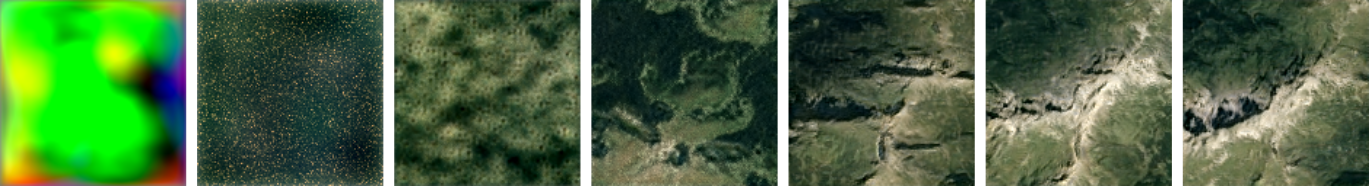
\includegraphics[width=0.95\textwidth]{RGB128Evo.png}
        \caption{Follows the progression of a vector after increasing epochs. From left to right: 0, 40, 80, 200, 320, 600, 1200 epochs.}
        \label{fig:RGB2500Evo}
\end{figure}

\subsection{128*128 RGBA Dataset}
The RGBA dataset adds the 4th elevation channel to the previous dataset. 
\subsection{On Quantitative Testing}
\section{Evaluation}
\subsection{Comparison Against Traditional Techniques}
\subsection{Further Work}
\subsection{Ethical Considerations}
\subsubsection{Data Ownership and Copyright}
The Google terms of service state that anything produced using their APIs must be attributed to them. Google is cited at multiple points in the work so while there is no worry of copyright infringement, it does bring up the larger issue of ownership of GAN-generated data.

The ownership and copyright of data produced by GANs is a heavily debated topic. One such notable copyright issue is the case of the Portrait of Edmond de Belamy \cite{ToDo}. This `painting' (figure \ref{fig:ToDo}) was generated by a GAN trained on 15,000 images of paintings by various artists over two different time periods. The result sold for \$432,500 at auction but there was heavy criticism about the artwork being available at the Christie's auction in the first place. Critics argued that the `artist', a group called \textit{Obvious}, did not deserve credit for the work.

The group had only recently started exploring AI for art generation in the past year and the GAN architecture they used had very limited input from them. \textit{Obvious} argued that because they selected the dataset for the model, they deserve credit for the work. None of the members of the groups identified as artists themselves, one was a computer science student and the other two business graduates. A prominent GAN artist, Mario Klingemann compared the artwork to a  `connect the dots children's painting', implying there was no real skill involved on \textit{Obvious}'s behalf.

In terms of this project, it could be argued that no real ownership is deserved here. The data all belongs to Google and the GAN architecture to NVIDIA. It could be argued however, that there is innovation in combining satellite and elevation data to train a GAN, and skill in the process involved. It is unlikely this same feat could be achieved with no significant research and practice in the area.

In any case, with ownership of GAN generated work still heavily contested, this project claims no ownership or copyright on the produced work. All training data is attributed to Google and the majority of the methodology to NVIDIA. The question of ownership of the resulting data is left for the viewer to determine. The data generated as part of this project serves only as an argument for the use of GANs for terrain generation. It is unlikely that anything produced using the code given alongside this dissertation could be of any use in commercial work, due to issues listed previously. Should this method or a similar method be employed, permission would need to be granted from Google for the use of their imagery, or at the very least an attribution made.

\subsubsection{Job Replacement}
Since technology's first introductions to the workplace, there have been fears surrounding job loss due to automation. One such example being the introduction of CAD/CAM, which led to fears of many draughtsmen losing their work \cite{ToDo}.

While Video Game development has always been inherently technology based, there are always manual tasks that can be reduced or made redundant by advancements in technology. With that considered, game developers often use this reduction in manual work as an opportunity to create bigger and better game worlds that would have taken years of work to develop previously. An example of this is Assassin's Creed Unity where designers used city blocks and styles to speed up the process of designing Paris \cite{ign_2014}.

If developing a commercial application of the methods produced in this paper, it is critical to evaluate how it would affect the work of game developers in the industry. The current methods of terrain development should be assessed to ensure the product would enhance the work of developers and not just replace it.

\section{Conclusion}
\subsection{Further developments}
\section{BCS Project Criteria and Self-Reflection}
\subsection{An ability to apply practical and analytical skills gained during the degree programme}
The fulfilment of this criterion is shown throughout the project. Modules such as \textit{Introduction to Artificial Intelligence} and \textit{Data Mining and Visualisation} taught me the technical background and theory to understand the basics of GANs and machine learning concepts. Throughout my degree I have practised researching skills and have shown this skill in action in the \textbf{Backgound Information} section of this dissertation. Good coding practice has been encouraged and rewarded in many of my modules and enforced the standard of the code produced as part of this project.
\subsection{Innovation and/or creativity}
I chose this project specifically for the opportunity to work on something creative and innovative. As previously mentioned, GANs are a relatively recent development and there is limited research into training them on combined satellite and elevation data. I would argue that having found only one other paper that follows a similar approach, the idea itself is innovative. 
\subsection{Synthesis of information, ideas and practices to provide a quality solution together with an evaluation of that solution}
\subsection{Project meets a real need in a wider context}
\subsection{Ability to self-manage a significant piece of work}
Self taught skills
\subsection{Critical self-evaluation of the process}
\renewcommand\bibname{References}
\bibliographystyle{IEEEtran}
\bibliography{refs}
\begin{appendices}
\subsection{Aims}
\begin{enumerate}
    \item Demonstrate the ability of a GAN to produce realistic and efficient\footnote{The definition of what constitutes realistic and efficient in this project is described in section 0.6} terrain elevation and rendering.
    \item Form a discussion that compares the effectiveness of a GAN technique to more traditional algorithmic techniques.
\end{enumerate}
\subsection{Objectives}
\subsubsection{Aim 1}
\begin{enumerate}
\renewcommand{\theenumi}{\alph{enumi}}
    \item Source satellite image and elevation data of the planet that is legally available for educational use.
    \item Source a sufficient amount of training data for the GAN to enable a fair comparison. The definition of a sufficient amount of training data for the discriminator would need to be defined in later stages of the project after initially testing the success of the model.
    \item Define a measure of success for the GAN.
    \item Develop a GAN with the aim of producing results that are indistinguishable by humans from those in the original data set. This objective is a desirable requirement of the model developed, however the closer the model is to reaching this standard, the better we are able to argue the merits of this approach. The process of developing a GAN will also increase my personal understanding of the subject and allow a more informed discussion.
\end{enumerate}
\subsubsection{Aim 2}
\begin{enumerate}
    \renewcommand{\theenumi}{\alph{enumi}}
    \item Outline the main similarities and differences between the use of GANs and traditional approaches to terrain generation.
    \item Form a meaningful argument. As this project is an investigation into how one technique compares to another, there is no bias to have a definite `winner'. To be classified as a meaningful argument, in line with the aforementioned article, this objective would be satisfied by completion of objectives c-f.
    \item Frame of reference: Define the context in which these techniques are being measured. For example, in the intended context of game design, it is worth noting why we would place more weight on the efficiency of the program at the expense of realism.
    \item Grounds for comparison: Explain the rationale behind the choice of terrain generation techniques used as examples in the project.
    \item Clearly define the relationship between the techniques: "Do they extend, corroborate, complicate, contradict, correct, or debate one another?" \cite{ToDo}
    \item Form the comparison around a clear organisational scheme.
    \end{enumerate}
\section{Spick and Walker: GAN Terrain}
\label{appendix:gan}
    \begin{figure}[H]
        \centering
            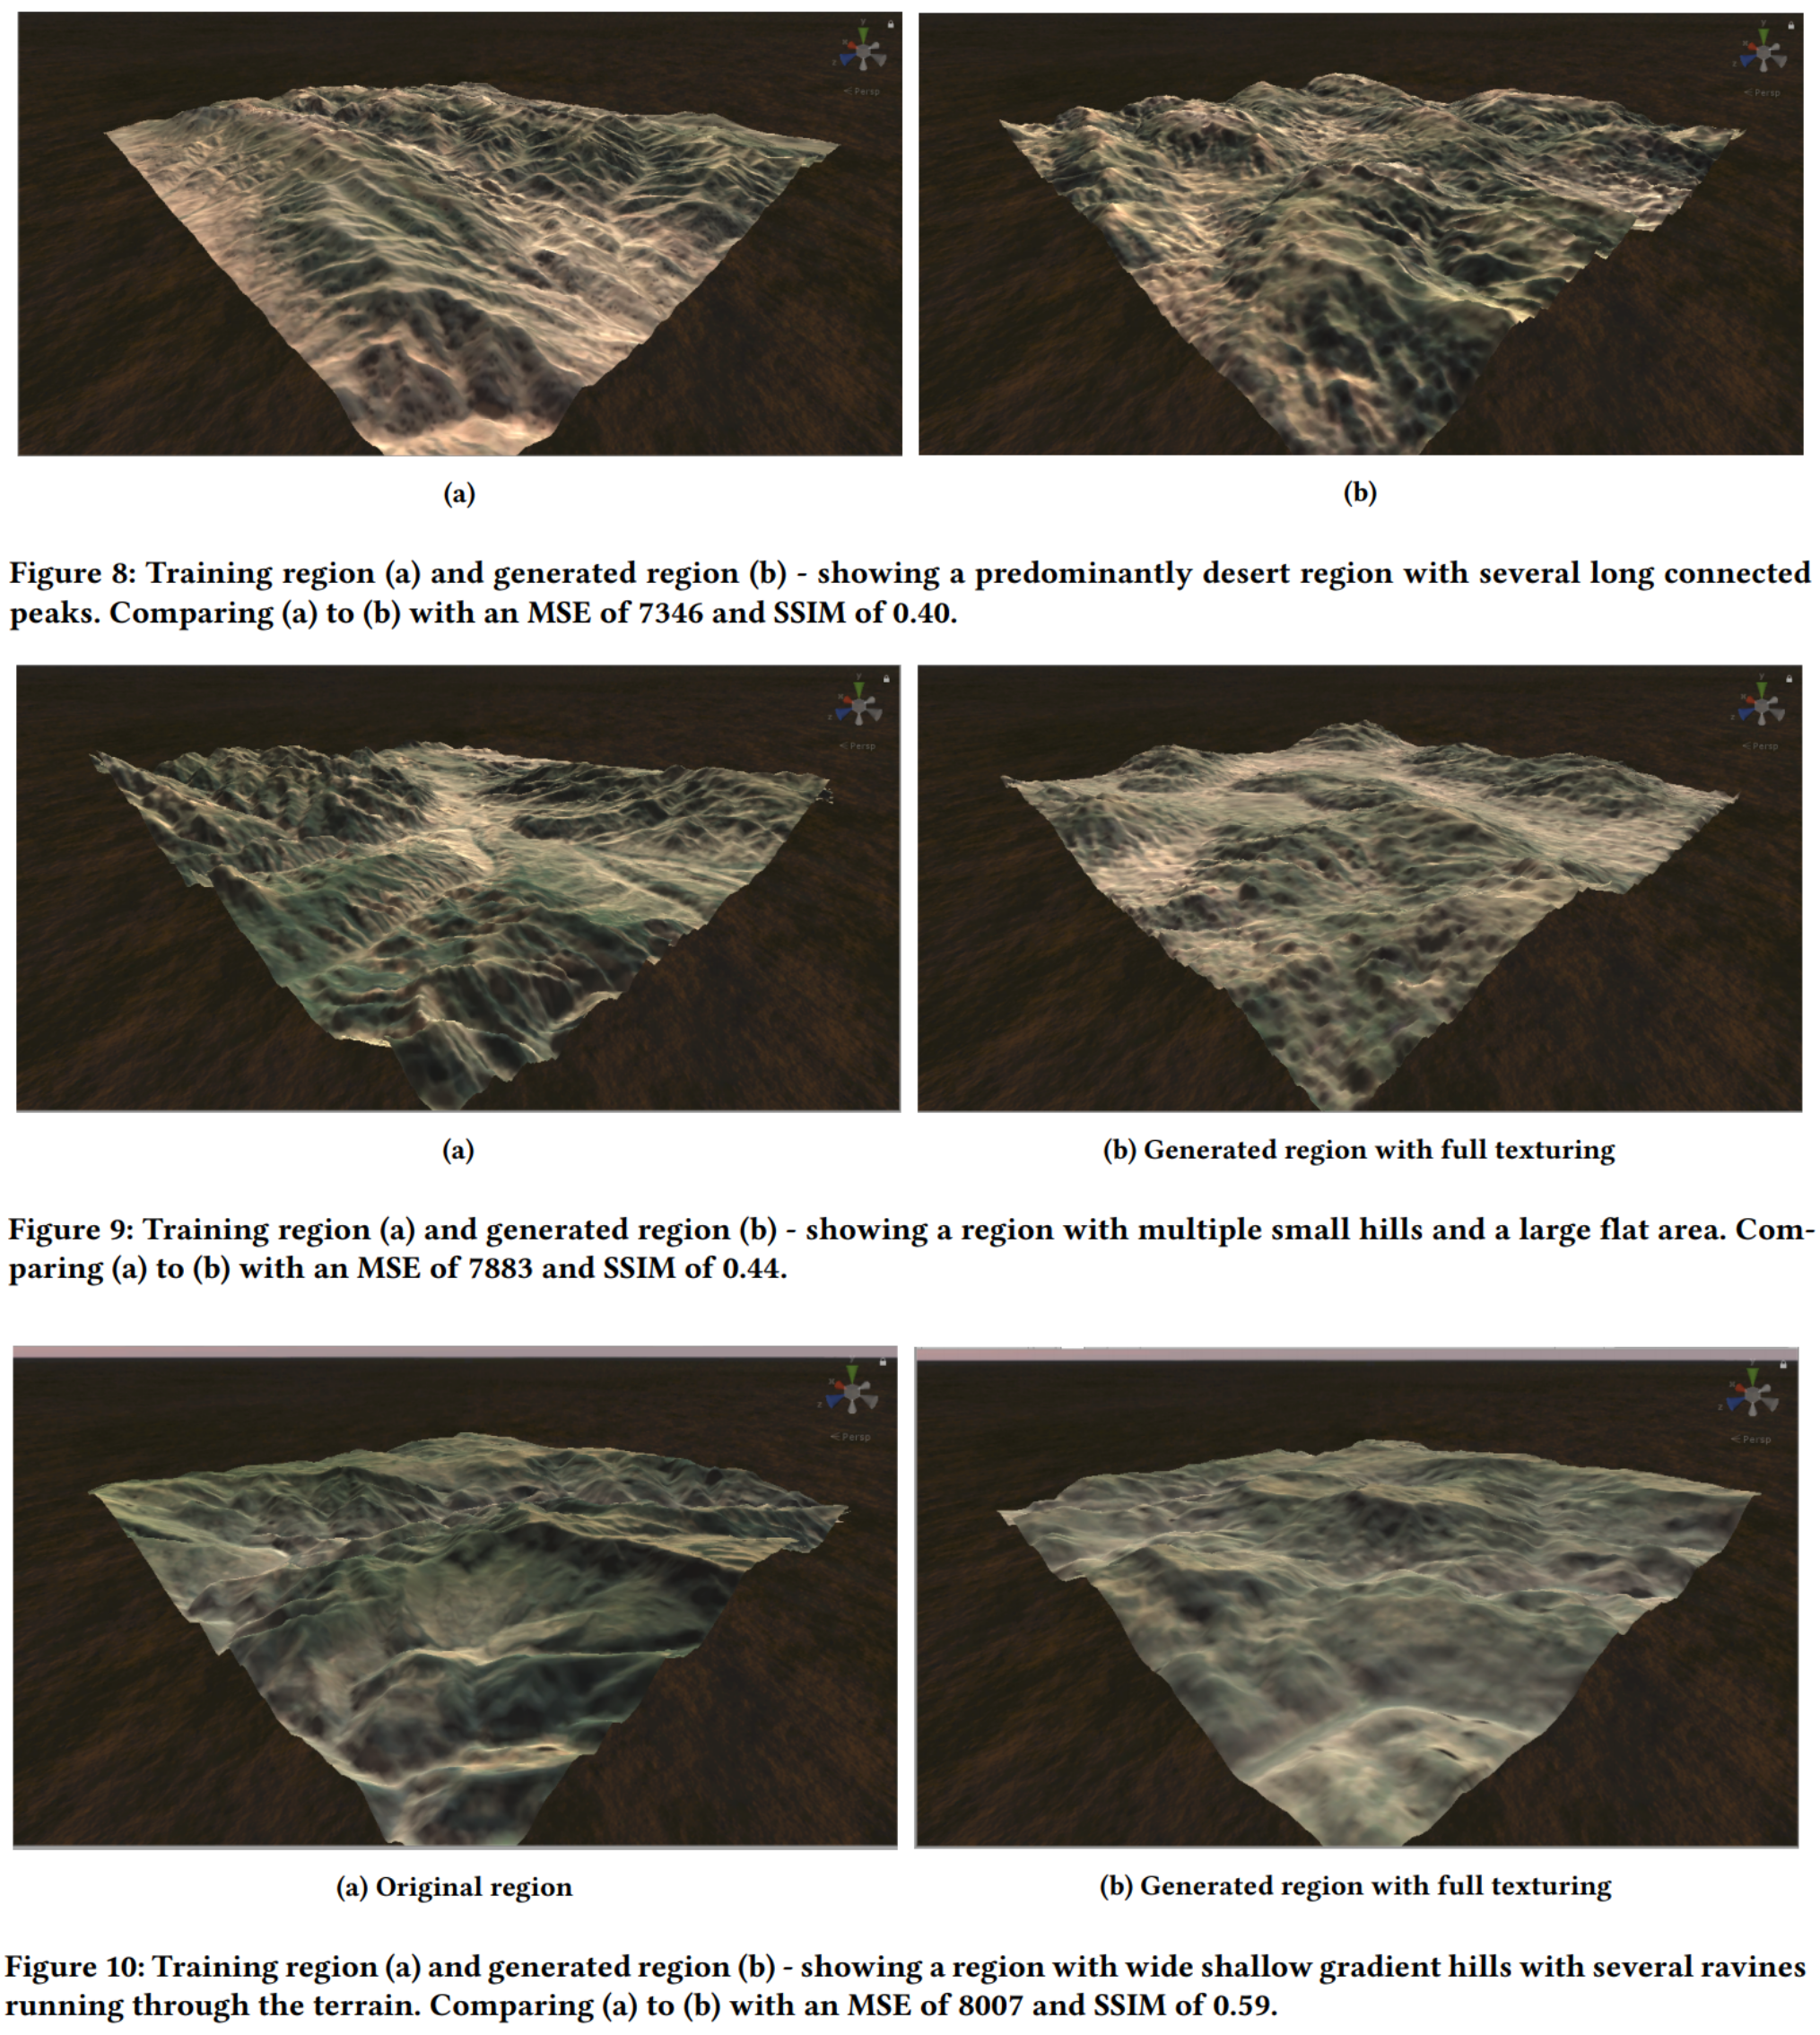
\includegraphics[width=0.9\textwidth]{evelRes.png}
            \caption{Shows the results of satellite river generation in \cite{riverSat}}
            \label{fig:elevRes}
    \end{figure}
\section{Code}
Code here?
\end{appendices}
\end{document}